\section{Micros-Switch Architecture}
\label{section:micros-awitch-architecture}
$\mu$SA, is designed for a logical target, unlike fixed pipeline of real target data planes with stationary processing blocks.
$\mu$SA provides multiple types of logical pipelines.
For each pipeline type, it exposes an interface type comprising a set of programmable blocks.
Programmers can define a P4 \texttt{package} type by implementing all the programmable blocks of a interface type.
In the same source file, programmers can provide multiple implementations of the same interface type to define multiple package types.
$\mu$SA pipelines do not have fixed-function blocks, instead it provides a set of logical externs which can be instantiated and used within control blocks of the $\mu$SA pipelines.
This design choice reduces heterogeneity in abstract model of data plane programs.

$\mu$SA defines various architecture specific structures and externs that allow programmers to express sequential and parallel composition of fine-grained packet processing functions.
It defines standard intrinsic metadata as~\texttt{msa\_sm\_t} as a struct type.
The fields of this struct provide basic information populated by the target e.g.,~\texttt{packet\_length}.
Some fields are not mutable, however $\mu$SA allows to declare instances of the struct and perform assignment operation between two instances to create copies.
Sections~\ref{subsection:pipelines} and~\ref{subsection:logical-externs} describe pipelines and logical externs, respectively.



\subsection{Pipelines}
\label{subsection:pipelines}
$\mu$SA has two types pipeline, Micro and Orchestration.
Figure~\ref{fig:msa-pipelines} shows programmable blocks of two types.
Micro pipeline interface comprises of parser, Micro-Pipe control and Deparser programmable blocks.
Every incoming packet is parsed and validated by the parser, if parser terminates in~\texttt{accept} parse state, then execution-control is transferred to micro-pipe control block.
Depending on use of logical externs in implementation, packet may not complete the processing of the control block.
If the execution-control reaches till the end of the control block, packet is processed by the deparser block.
\begin{figure}[!ht]
    \begin{subfigure}{0.45\linewidth}
        \centering
        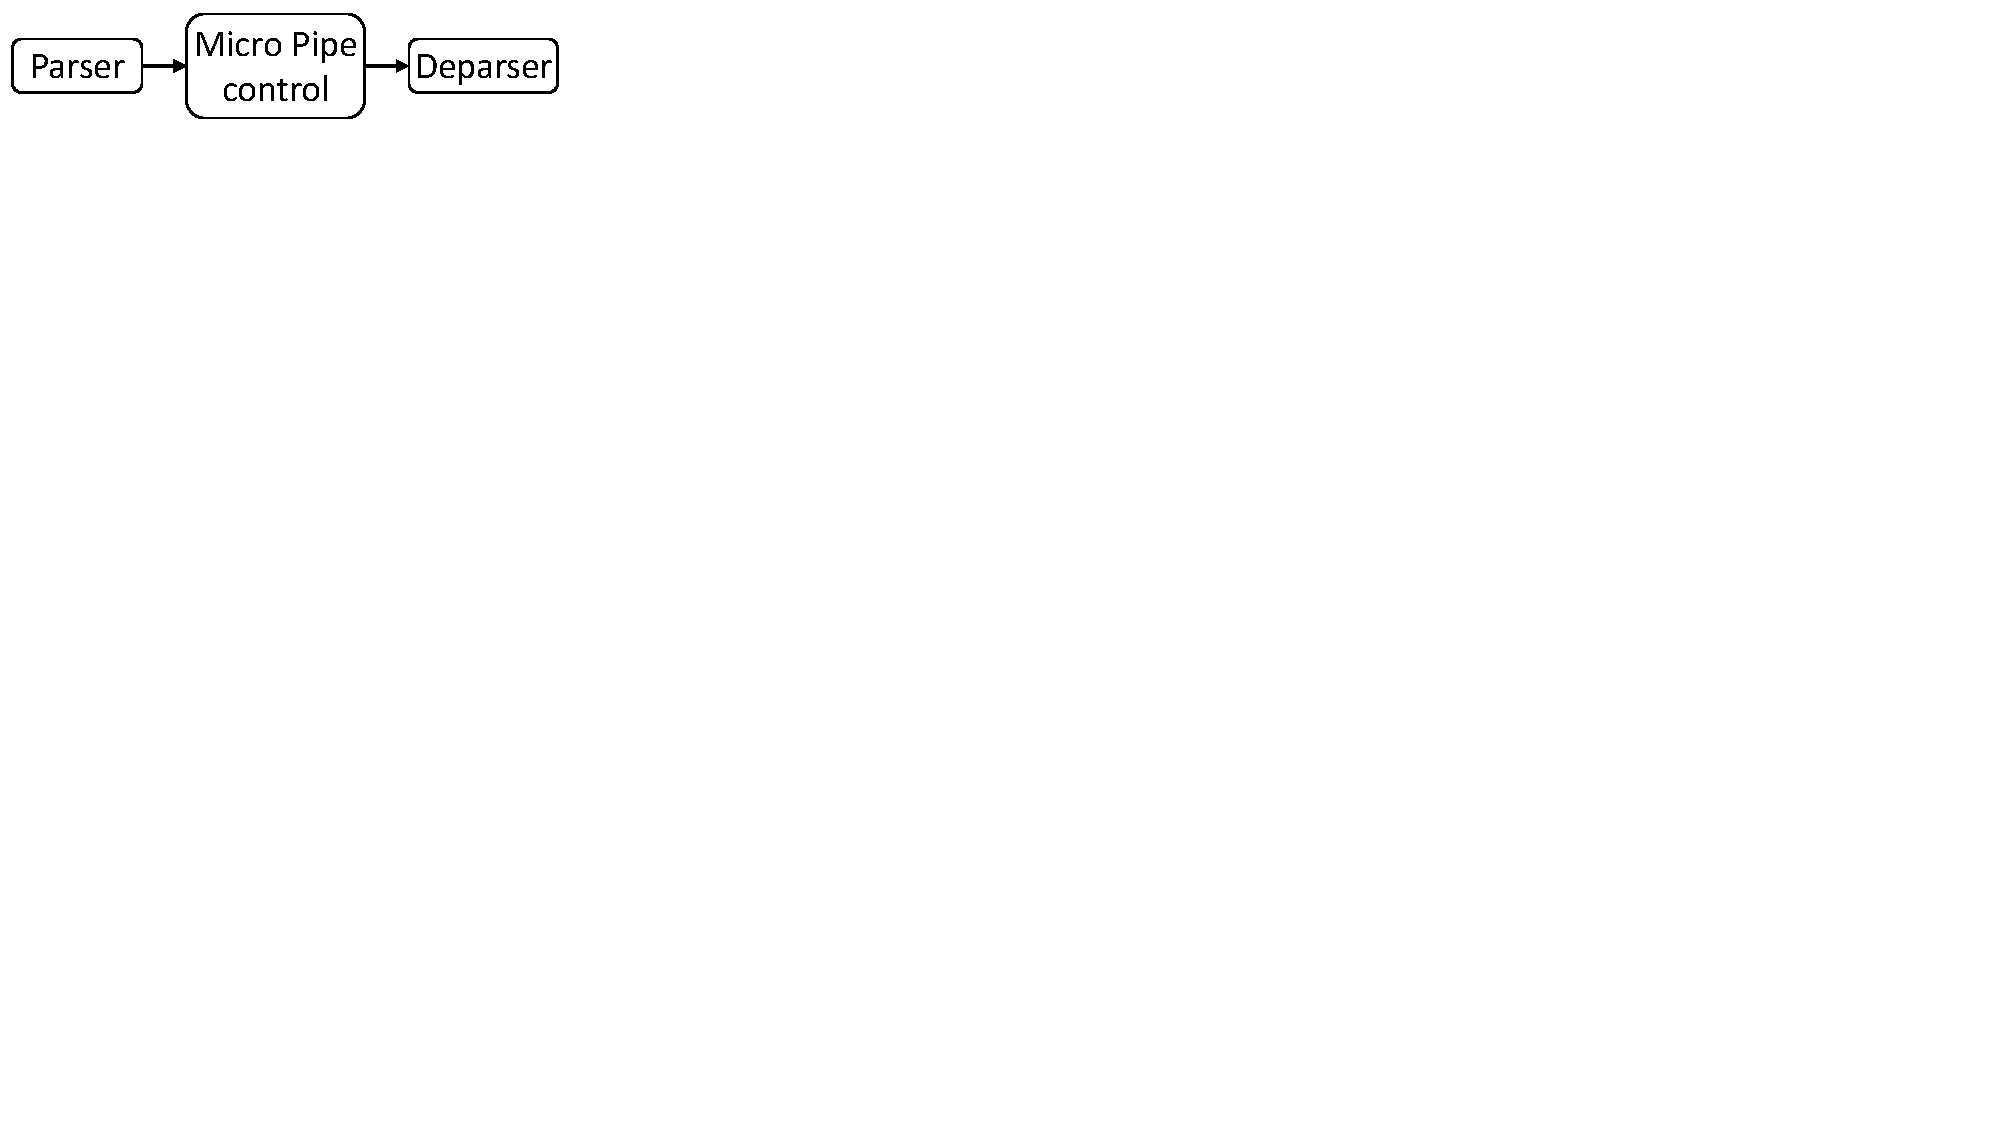
\includegraphics[trim=0 482 692 0, clip,scale=0.45]{msa-pipeline}
        \caption{Micro}
        \label{subfig:micro}
    \end{subfigure}
    \begin{subfigure}{0.45\linewidth}
        \centering
        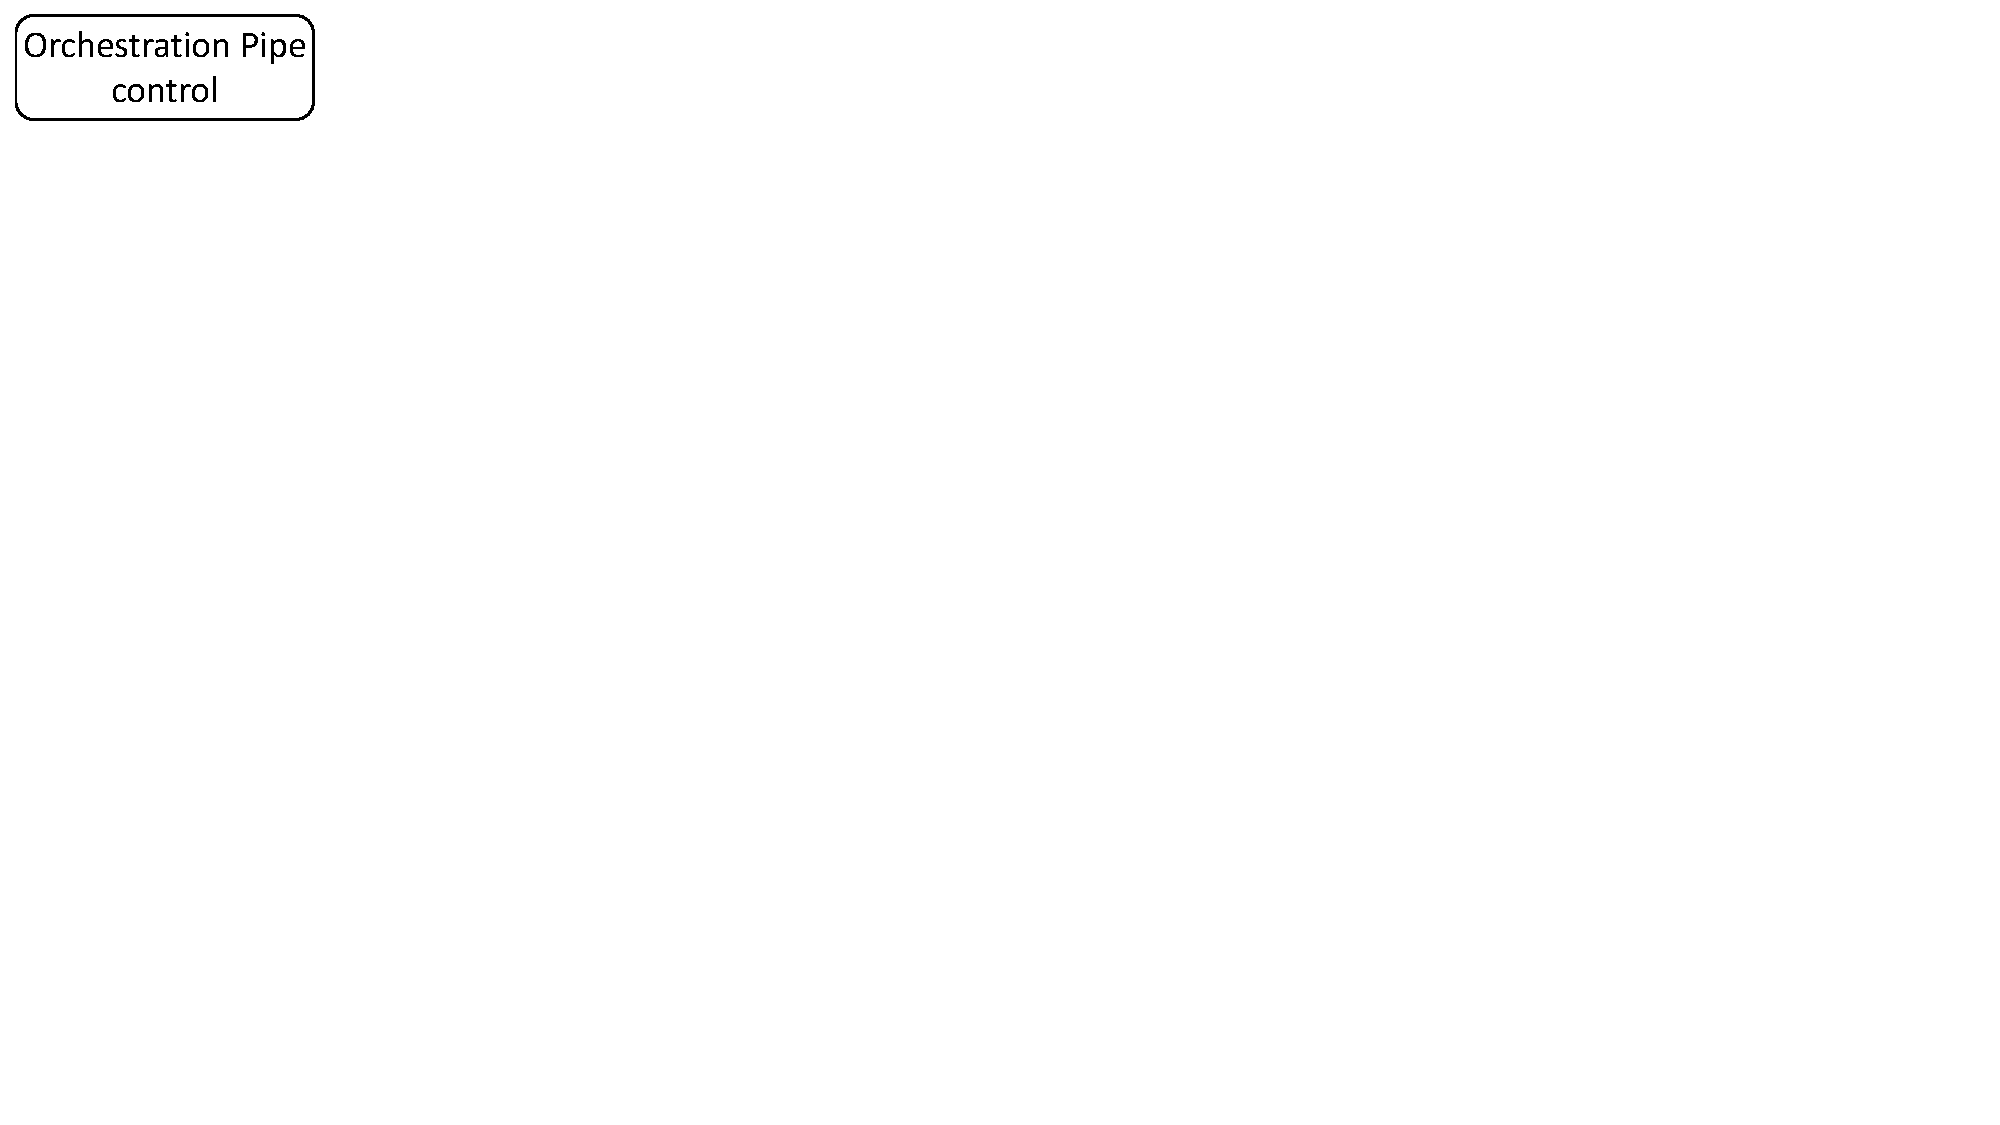
\includegraphics[trim=0 480 805 0,clip,scale=0.45]{micro-orchestration-pipeline}
        \caption{Orchestration}
        \label{subfig:orchestration}
    \end{subfigure}
\caption{$\mu$SA Pipelines}
\label{fig:msa-pipelines}
\end{figure}

Orchestration pipeline interface has only a control block, orchestration pipe.
Programmers can implement imperative control flow using intrinsic metadata of $\mu$SA and runtime parameters to the package types.
In addition of existing language features, it allows programmers to instantiate package types and invoke them in the body(~\texttt{apply}) of the control block.



% \begin{figure*}
% \noindent \begin{minipage}[t]{\linewidth}
% \begin{lstlisting}[frame=none]
% 
% Orchestration<I, O, IO, U, R>(msa_packet_in b, msa_packet_out po, inout msa_sm_t sm, egress_spec es, in I iargs, out O oargs, inout IO ioargs) ()
% 
% MicroSwitch<I, O, IO, U, R>(msa_packet_in b, msa_packet_out po, inout msa_sm_t sm, egress_spec es, in I iargs, out O oargs, inout IO ioargs) ()
% 
% \end{lstlisting}
% \end{minipage}
% \vspace*{-10pt}
% \caption{$\mu$SA Pipeline Interface Types}
% \end{figure*}


\subsection{Logical Externs}
\label{subsection:logical-externs}

TODO rename ``function'' to ``mehod''.
\subsubsection{Packet Externs}
Packets are represented using \texttt{packet\-\_in} and \texttt{packet\_out} externs defined in P4-16 core library~\cite{core.p4}.
However, these externs do not provide functions and semantics required to describe sequential and parallel composition of programs.
We define $\mu$SA specific packet externs to allow programmers to express sequential and parallel processing. 
$\mu$SA specific packet externs \texttt{msa\_packet\_in} and \texttt{msa\_packet\_out} contain an instance of \texttt{packet\_in} and \texttt{packet\_out}, respectively.
We introduce a function, \texttt{get\-\_packet\-\_in}, in \texttt{msa\-\_packet\-\_out}.
\begin{lstlisting}[frame=none]
void get_packet_in(msa_packet_in msa_pin);
\end{lstlisting}
Similarly, we introduce copy\_from function in \texttt{msa\_packet\_in} that replicates the state of passed argument (\texttt{msa\_pin}) to the calling instance.
\begin{lstlisting}[frame=none]
void copy_from(msa_packet_in msa_pin);
\end{lstlisting}
\subsubsection{Egress Specifications}
To support special features, the architectures of real target devices provide intrinsic metadata  that depends on operations on other intrinsic metadata.
For example,  many real targets allow to measure every packet's queuing latency through the device.
The queuing latency is computed by recording enqueue and dequeue timestamps in the device.
These timestamps can be measured only after the packet's egress port is finalized and the packet is sent to the packet buffer.
The architectures of real target devices expose timestamps as intrinsic metadata which can be accessed only after the egress port is finalized.
\begin{figure}[!h]
\begin{lstlisting}[frame=none]
enum msa_metadata_t {
  INGRESS_TIMESTAMP,
  EGRESS_TIMESTAMP
}
extern egress_spec {
  void set_egress_port(in bit<8> port);
  bit<8> get_egress_port();
  bit<32> get_value(in msa_metadata_t ft);
  void copy_from(egress_spec es);
}
\end{lstlisting}
\caption{Egress\_Spec Extern}
\label{fig:msa-egress-spec-extern}
\end{figure}
$\mu$SA considers \texttt{egress\_spec} as a stateful extern object (Figure~\ref{fig:msa-egress-spec-extern}) providing functions to set and get \texttt{egress\_port} and retrieve values of other egress\_port dependent intrinsic metadata.
$\mu$P4C allows repeated usage of the extern's functions in the single control block of $\mu$SA pipelines.
$\mu$P4C uses their occurrences to transform the code to multi-control pipelines of real target architectures.
If \texttt{get\_value} occurs before \texttt{set\_egress\_port} on any possible execution-control path, $\mu$P4C raises a compile-time error.

\subsubsection{Packet Buffer}
$\mu$P4 allows programmer to express parallel processing of multiple P4 programs by passing the copy of the packet and intrinsic metadata to multiple programs.
Programmers can use assignment statements to create copies of standard intrinsic metadata (msa\_sm\_t) and use~\texttt{copy\_from} functions in~\texttt{msa\_packet\_in} and~\texttt{egress\_spec} to create copies of the packet and intrinsic metadata.
In addition, it provides logical a packet buffer as an extern (Figure~\ref{fig:msa-packet-buffer-extern}) to serialize output packet and intrinsic metadata.
The logical buffer extern can only be instantiated in the control block of orchestration pipeline.
Its functions can be used only in apply body of the control block.
The output of the multiple programs generated by processing the same packet can be enqueued in the logical buffer.
The dequeue function allows to fetch the packets and either pass it to another program to process or assign it to the msa\_packet\_out argument of orchestration pipe control block.
\begin{figure}[!h]
\begin{lstlisting}[frame=none]
extern msa_packet_buffer<ET> {
  msa_packet_buffer();
  void enqueue(msa_packet_out po, in msa_sm_t sm, egress_spec es, in ET data);
  void dequeue(msa_packet_in pin, out msa_sm_t sm, egress_spec es, out ET data); 
}
\end{lstlisting}
\caption{Packet Buffer Extern}
\label{fig:msa-packet-buffer-extern}
\end{figure}
\subsubsection{Multicast Extern}
$\mu$SA's multicast extern (Figure~\ref{fig:msa-multicast-extern}) can be instantiated in the control blocks of its pipelines.
The \texttt{set\_multicast\_group} can be used to assign replication group to the packet. 
The \texttt{apply} function is allowed to use only in \texttt{apply} body control blocks. 
It is analogous to~\texttt{fork} system call in C except that processing of original packet terminates at the apply call.
It returns instance id of the replicated packets and populates the egress\_spec instance with the port id set by the control plane.
$\mu$P4C translates this extern to multicast mechanism defined in architectures of real targets.
We assume these architectures would have sufficient fields to program their replication engine, so that a combination of the fields can be used as packet instance id.
\begin{figure}[!h]
\begin{lstlisting}[frame=none]
extern msa_multicast_engine {
  msa_multicast_engine();
  void set_multicast_group(GroupId_t gid);
  PacketInstanceId_t apply(egress_spec es);
}
\end{lstlisting}
\caption{Multicast Extern}
\label{fig:msa-multicast-extern}
\end{figure}
